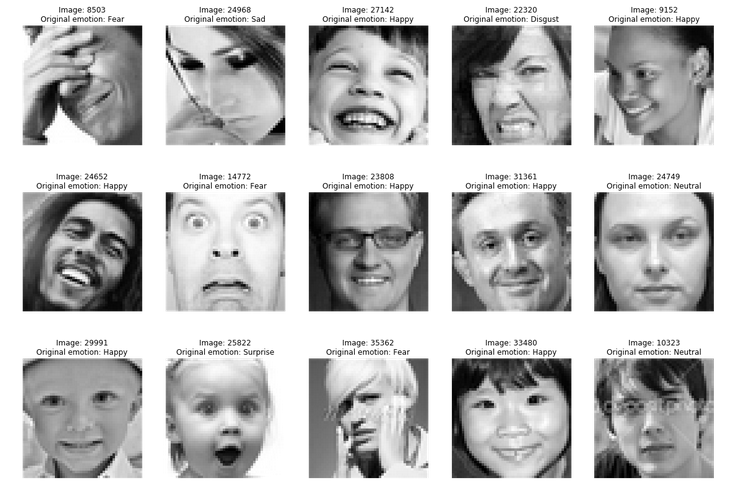
\includegraphics[scale=0.75]{images/ferCover.png}
\\Data that we got is in one *.csv ~\cite{kaggleFER} file with almost 36 thousands rows and two columns. The data consists of 48×48 pixel gray scale images of faces. The faces have been automatically registered so that the face is more or less centered and occupies about the same amount of space in each image.
\\Columns contain:
\begin{itemize}
  \item number of emotion \\
        in range 0 - 6
        \begin{itemize}
          \item 0 - angry
          \item 1 - disgust
          \item 2 - fear
          \item 3 - happy
          \item 4 - sad
          \item 5 - surprise
          \item 6 - neutra
        \end{itemize}
  \item string of pixels \\
        pixels are in one long string (2304 of them), they are in grayscale 0 - 255.\\
\end{itemize}
This pixels will be processed depending on the model.\\
Training part has 28708 images, testing only 7178.